\documentclass[11pt, letterpaper, oneside, twocolumn]{article}
\usepackage{fancyvrb}
\usepackage{float}
\usepackage{subfig}
\usepackage{graphicx,dblfloatfix}
\usepackage[hmargin=1in, vmargin=1in]{geometry}               
\usepackage{enumitem}
\usepackage{tikz}
\usetikzlibrary{arrows,backgrounds,calc,fit,mindmap,positioning,trees,shapes}
\usepackage{xcolor}

% \usepackage{fullpage}
% \usepackage{xunicode,xltxtra,url,parskip} 	%other packages for formatting

% \addtolength{\topmargin}{-.5in}
% \addtolength{\bottommargin}{-.875in}
% \addtolength{\textheight}{1.75in}

\setitemize{noitemsep,topsep=0pt,parsep=0pt,partopsep=0pt}
\DefineVerbatimEnvironment{code}{Verbatim}{fontsize=\small}

\newcommand{\tab}{\hspace*{2em}}
\floatstyle{plain}
\restylefloat{figure}
\begin{document}
\title{Yippee: Web Search for the New Millenium}
\author{	TJ Du, Chris Imbriano, Margarita Miranda, Nikos Vasilakis\\
	\{tdu2, imbriano, mmiran, nvas\}@seas.upenn.edu}
\date{May 8, 2012}

\maketitle

\label{sec:SOAR} %software architecture
\begin{figure*}[ht]
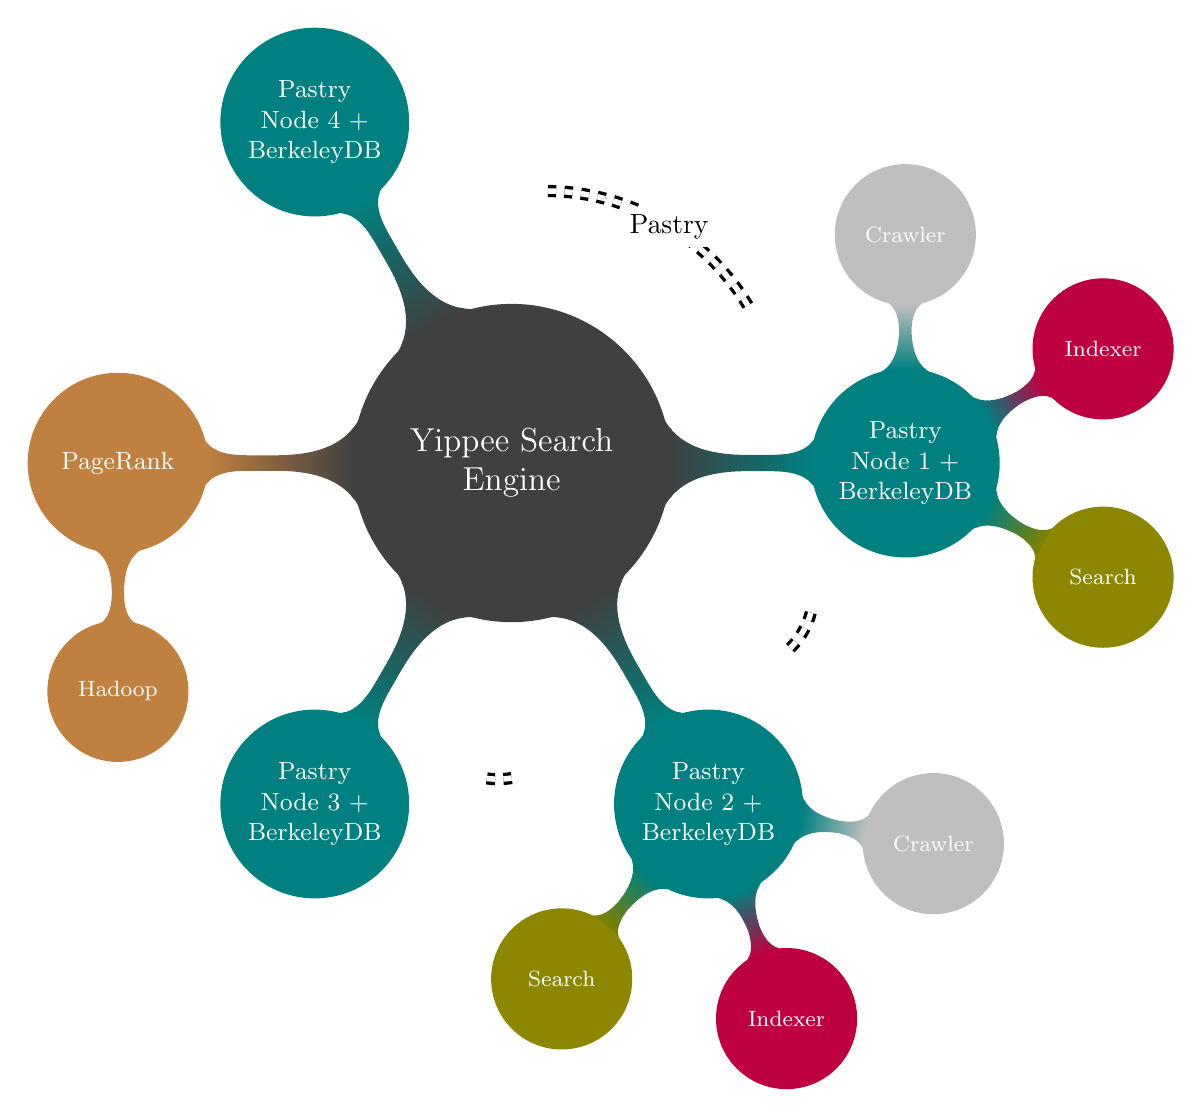
\begin{tikzpicture}
  \path[mindmap,concept color=darkgray,text=white]
    node[concept] {Yippee Search Engine}
    [clockwise from=0]
    child[concept color=teal!] {
      node[concept] {Pastry Node 1 + BerkeleyDB}
      [clockwise from=90]
      child [concept color=lightgray!] { node[concept] (c1) {Crawler} }
      child [concept color=purple!]  { node[concept] (i1) {Indexer} }
      child [concept color=olive!] { node[concept] (s1) {Search} }
    }  
    child[concept color=teal!] {
      node[concept] {Pastry Node 2 + BerkeleyDB}
      [clockwise from=-10]
      child [concept color=lightgray!] { node[concept] (c2) {Crawler} }
      child [concept color=purple!] { node[concept] (i2) {Indexer} }
      child [concept color=olive!] { node[concept] (s2) {Search} }
    }
    child[concept color=teal!] { node[concept] {Pastry Node 3 + BerkeleyDB} }
    child[concept color=brown!] {
      node[concept] {PageRank}
      [clockwise from=-90]
      child { node[concept] {Hadoop} }
    }
    child[concept color=teal!] { node[concept] {Pastry Node 4 + BerkeleyDB} };

    \begin{pgfonlayer}{background}
        % \draw [circle connection bar ] (i1) edge [color=violet!50!] (i2);
        % \draw[-to,shorten >=10pt,gray] (c1) -- (c2);
        \draw[very thick, dashed, double distance=2pt] (3,2) arc (31:90:3cm);
        \draw[very thick, dashed, double distance=2pt] (3.8,-1.9) arc (-15:-50:1cm);
        \draw[very thick, dashed, double distance=2pt] (0,-4.0) arc (-80:-100:1cm);
        %\node[anchor=north,text width=10cm,inner sep=.05cm,align=center,fill=white] at (2,2) {Pastry}; text width=3cm,
        \node[fill=white, inner sep=0.1cm, text centered] at (2,3) {Pastry};
    \end{pgfonlayer}
\end{tikzpicture}
  \caption{Yippee's fully distributed architecture. Nodes communicate
  via FreePastry}
\end{figure*}

\section{ Introduction }

To say the world wide web is enormous would be an understatement.  
In the last month (March 2012),  Google's index size was estimated to be between forty-five and fifty-five billion pages.\cite{websize}
The task of presenting a web user with relevant pages according to keyword search has proven to be a difficult one, as many of the commercial search engines during the dawn of the web were unable to return their own site for a search for their site's name.\cite{google} 
Google has shown that besides the load speed of the results, page relevance is just as critical a metric of an effective search engine. 

Yippee is a distributed search engine designed to provide fast, relevant results to keyword queries via the web.  

\section{Project Approach}
\label{sec:approach}

The Yippee Search Engine is a distributed application comprised of 4 main components: a web crawler to recursively download pages from the web, an indexer to index crawled web pages, our simplistic implementation of Google's PageRank algorithm \cite{pagerank}, and a search module to retrieve documents based on user-provided keywords.  
The crawler, indexer and search components are distributed via the FreePastry peer-to-peer substrate, while the PageRank components is centralized.  All parts of the project are deployed to Amazon Elastic Cloud Computing (EC2) instances.  

The architecture of the Yippee is shown in figure 1.



Section \ref{sec:component} will describe each component and its relevant design decision.
Section \ref{sec:evaluation} will present evaluations for some of the design decisions. \textbf{rephrase}

\section{Component Discussion}
\label{sec:component}

\subsection{Infrastructure and Software Engineering}

We used four Extra Large (m1.xlarge) Amazon EC2 instances, each comprised of eight 4-core CPUs, 15GB of RAM.
To each instance, we attached a one terabyte Elastic Block Storage volume. 
Yippee was implemented using Java 1.6 and the user-interface servlet adhered to the Servlet API 2.4 specification. 
Ant (v. 1.8) and bash scripts were used to automate the build, test and deployment process, allowing us to start any combination of componets in any mode (test, integration and production) with simple command-line arguments.
We practiced test-driven development \footnote{We used jUnit 4, instead of 3, mainly due to flexible fixtures.} while pair-programming each component.  Each pair was responsible for implementing white-box tests for the component they implemented, while the other team wrote black-box tests (and vice versa). 
The project was version controlled with git (v. 1.7.4) and shared among team members via Github.
At the time of submission, there are approximately 14k lines of code in the Yippee source and test directories.

Yippee uses BerkeleyDB for persistent storage and as an asynchronous queue between components (such as the crawler and the indexer). In this way, the crawler could start and stop at any time without affecting the indexer and page-rank.  

In order to route data across multiple nodes, we made use of FreePastry, a Pastry implementation. 
Pastry is an overlay and routing network for the implementation of a distributed hash table(DHT) similar to Chord. 
All packages share a common singleton object for configuration, which made it easy to access get and receive messages of different priority. 
Each message is sent by the module responsible for routing messages, and handled accordingly upon retrieval.

\subsection{Crawler}

The Yippee crawler is a multithreaded distributed crawler based on the design of the Mercator crawler\cite{mercator}. 
Each of the Yippee node is responsible for a subset of the web as determined by FreePastry key-based routing keyed on the host of each url discovered.
Mercator uses various implementations of the URLFrontier to fine tune the crawlers performance and politeness.
The crawler is multithreaded and requires very little inter-thread communication, but the URLFrontier can be a bottleneck depending on the implementation. 
Given the critique of the centralized nature of Mercator's URLFrontier \cite{ubi, para}, we made our frontier pluggable via a factory pattern to allow easy testing of frontiers with varying degrees of politeness and speed.

The Yippee Crawler has three important persistence structures; DocAug, FrontierSavedState and RobotsTxt.
DocAugs are wrapper objects for the contents of the crawled documents, augmented with a number of metadata (such as date and url).
They are an object stored by the crawler and later read by the indexer.
FrontierSavedStates store the necessary data to checkpoint the state of a URLFrontier and allow for restarting a frontier without losing the URLs waiting in the queue.
Last is the RobotsTxt object which stores information retrieved from the robots.txt file for a given host.
The RobotsTxt interface is defined such that the object can take a url as a parameter and determine if the robots.txt policy allows crawling.

Though Yippee deployed only four EC2 instances, financial obligations to Amazon not-withstanding, there is no reason that prevented us from deploying more nodes.
More crawling nodes would result in more pages crawled per unit time, however, we did experience a bottleneck as a result of too many Pastry messages.
In the case we saw, upgrading the Amazon instance to a more powerful instance helped resolve that bottleneck to a degree.
It is not clear, without some experimentation, whether more crawling nodes would help the bottleneck by reducing the message handling load of an individual node, or the added pages being crawled would increase the number of urls distributed and have the opposite effect.

The Yippee crawler is resilient to failure in that if a node dies, the urls that would have been routed to it are directed to the next available node, per FreePasty's routing.
The Yippee application does not however maintain duplicate data, so any already crawled pages, or discovered urls, will be lost and need to be crawled again.
We felt these tradeoffs were reasonable given the timeline and scope of the project

\subsection{Indexer}

The Yippee Indexer has a multi-threaded and distributed design loosely based on Google's  PageRank algorithm\cite{pagerank}. 
The Indexer on each node creates IndexerWorker threads that then perform all work. 
All IndexerWorkers poll from a queue of documents that are placed into the BerkeleyDB DocAug database by the Crawler. 
JTidy is used to parse each document. 
For every word in the document, the Porter Stemmer algorithm is used and the stemmed word is compared to a Lexicon of stemmed words and a regular expression to look for numbers. 
If the word is valid, a Hit object is created. 
The Hit object contains important information about that word in relation to the document: document id, document length, position, and word decoration (bold, italics). 
Similarly, any anchor hit on a document gets created as both a Hit for that document and an AnchorHit for the document its link refers to. 
An AnchorHit object is an extension of the Hit object and includes a field for the document it points to. 
The decision to create both a Hit and an AnchorHit for an anchor was based on the fact that the word tells very important information about both documents. 
At this point the link of the current document getting indexed and the link found get logged to a special file that will later get used for PageRank. 
After all the Hit and AnchorHit objects are created for that document, two things happen. 
First, a DocEntry object is created and saved to the DocEntry Database. 
This object contains valuable information about the document needed pre- and post-query such as page rank, tf-idf, document url, and document title. 
Second, all the Hits for that document are sent to a centralized NodeIndex that handles them.


The NodeIndex accumulates all the Hits into a HashMap that stores the word as its key and an ArrayList of Hits for that word from all IndexWorkers. 
The Hits will get saved in a Barrel database on the node whose id is closest to the Hit's SHA-1 hashed word. 
FreePastry is used for passing the ArrayList of Hits for a word to the appropriate node. 
In order to reduce the number of messages being passed around the pastry ring, messages were sent in batches. 
For every 10 documents whose Hits were sent to the NodeIndex, the current HashMap would get iterated over and only words whose ArrayList of Hits were longer than 3 would get sent to the ring to get saved in the Barrels. 
These values were chosen based on finding a balance with the frequency and size of the Pastry messages being sent. 


The Barrels contain an inverted index and is managed by a BarrelManager. 
There is a BarrelManager on each node that is responsible for the HitLists of all the words whose ids get hashed to it. There is only one HitList object for every word. 
A HitList contains the word, document frequency, and two HashMaps: one for Hit term frequency and another for AnchorHit term frequency in a particular document. 
The keys for the HashMaps are the document ids and the values are floats. 
Upon message arrival, a HitList object is either created or updated depending on whether that word has been seen before. 
Then document frequency and term frequency are adjusted accordingly. 
This is performed at this point in order to reduce the number of calculations done post query search.  

\subsection{PageRank}

The PageRank component of Yippee is the only centralized part of the system.
It performs a calculation based-on PageRank algorithm\cite{pagerank} to determine the relative importance of each page in the index.
The PageRank calculation is an iterative MapReduce process running on a single-node Hadoop cluster after retrieving, from each Yippee node, a log of links found during the indexing process.
We decided that PageRank should not be a distributed component for a number of  reasons. 
First, the PageRank metric is only relevant when doing searches and since the Yippee Search Engine would only be in deployment for a short period of time, it was not necessary to run PageRank multiple times in our production environment.
Second, given the frequency of PageRank jobs, implementing a distributed version introduced complexity that was unwarranted, so the simpler solution was chosen.

\subsection{Search}
The final piece of Yippee involves presenting the user with relevant pages given a user-provided keyword.
The search component of the Yippee Engine utilized the Barrel and DocEntry indices to retrieve and aggregate statistics for calculating the TF-IDF ranking. 
Search queries were split by word and distributed to the appropriate node via key-based routing. 
If the word was found to have Hits in the corpus, all documents matched in that HitList are retrieved from the ring (via key-based routing again.) 
If a word had no matches or was not found in the lexicon, a null reply message is sent immediately, to notify that no results will be returned. 
Once all DocEntry objects have been aggregated on the query node, we were able to continue onward to ranking the documents. 
Of note, each query is assigned a unique queryID such that messages sent and replied would be associated with the correct query. 
This way, the search functionality has high scalability without losing integrity. 
Additionally, cached queryIDs paved way for future work in caching results and iterating through pages of results.
As for ranking matched documents, we used the TF-IDF and PageRank values to calculate ranking scores for all documents. 
The TF-IDF value of a document was calculated as the product of the sum of its weighted text frequency(tf) and anchor text frequency(atf) values. 
In this case, the atf values were anchor text hits from other pages pointing to the current document. For each document we weighted its tf by 0.4 and the atf by 0.6 because we felt that given the implications of PageRank link analysis, that the content of a given page may be more accurately described by links point to it. 
Finally, once all hits per document are summated, each document's TF-IDF value was then multiplied by the PageRank value (default of 1) to give the final rank value. 
The documents were then sorted by descending value and returned in a list.
The results returned are then displayed with statistics on search time elapsed and the total number of documents matched.

\section{Evaluation}
\label{sec:evaluation}

Crawler eval - mention corpus size of the weekend ~75k docs

The Indexer performed best with 5 IndexerWorker threads at a rate of 250 documents per minute. 
This is timed from when the document is polled from the queue by the IndexerWord to when the Hits are saved to the appropriate Barrels. 
Increasing the number of threads resulted in Pastry messages getting sent out more frequently and overflowing the node queues. 
There was also overhead in writing to the DocEntry database between the threads. 
Despite this, the performance rate over time was constant meaning overflow of messages was eliminated. 

The search data displayed in FIGURE-SEARCH were generated by searching a series of three letter words, on a single node cluster.
The pattern we observe is that the amount of time required by the search increased in a linear fashion.
These data indicate a design issue in the way we indexed documents in a distributed manner: the more results we matched, the more documents we needed to collect before we were able to rank.
We believe though the time increases linearly in our data, given calculation and data transfer, the rate would eventually slow down dramatically, even despite adding more nodes.
Unfortunately, since the size of our corpus never exceeded 10k documents, the search time never exceeded 1s in elapsed time and the issue went unnoticed.
In order to fix this issue, we could have implemented a more distributed ranking implementation, such that 

PageRank seems to scale well at input size below one million links.
As mentioned, our indexed corpus never got too large and so we never ran PageRank on input sizes greater than about 350k links.
We combined input from numerous crawl/indexes to generate sample data for figure (GRAPH NUMBER).
Unfortunately, the pagerank process repeatedly failed for an input size of one million, suggesting perhaps we either needed even more computing power to perform the calculation in a centralize manner, or a dis

\section{Future Work}
\label{sec:future}

Given more time and budget, we would focus improvement efforts in the areas of scalability and robustness to improve corpus and index size.
Additionally, implementing a Mercator style URLFrontier more closely to the original would provide us with a much more polite crawler. 
Search efficiency could be improved with better caching techniques for queries.
For result improvement, we will implement spell-check, user feedback on query results, and context/phrasing taken into account for queries. 
We would also be working with a larger corpus.
Other features we will also implement is a way to update Hit objects when a document is crawled again and the contents have changed.


\section{Conclusion}
\label{sec:conculsion}
Overall, we feel that this project was a success.
Despite a few shortcomings, we were able to build a sophisticated search engine which is stable and efficient.

The multi-threaded indexer component was very stable and indexed pages efficiently without much decrease in performance with respect to corpus size.
Since our indexer used FreePastry to store its indices, it would have scaled very well with respect to more nodes.
On the other side of this, the indexer was limited when nodes were few due to the high number of messages sent to the ring.
Thus we learned that when a great amount of data must be distributed around a ring, with fast speed, we need to consider expanding the size of the ring to accommodate the data.

The search component was stable and efficient as well, and ranked results fairly well. Though we had a limited corpus, when we queried items contained within the corpus, the result was fast and usually within 1-5 spots of the top ranked spot. Since we weighted anchor hits more heavily than text hits, it was difficult to tune these metrics without a more robust corpus. Pages with more coverage tended to be ranked higher in relevance, whereas other with less coverage were left with a lower score. Had we more time, we would have hoped to crawl a larger corpus and better tune this metric. Perhaps anchor hits would be better off being weighted less, since they are subject to connectivity. Regardless of the ideal algorithm, we tuned ours to give the best results possible with our limited data, and we feel that the results returned were of good quality, despite our shortcomings.




\begin{thebibliography}{9}

  \bibitem{websize} WorldWideWebSize.com, 11 Apr 2012 $\langle$http://www.worldwidewebsize.com$\rangle$
  \bibitem{google} Sergey Brin and Lawrence Page \emph{The Anatomy of a Large-Scale Hypertextual Web Search Engine}, Stanford University, 1999
  \bibitem{pagerank} Sergey Brin and  Lawrence Page and Rajeev Motwani and Terry Winograd \emph{The PageRank Citation Ranking: Bringing Order to the Web}, Stanford InfoLab, 1999
  \bibitem{mercator} Allan Heydon and Marc Najork, \emph{Mercator: A scalable, extensible web crawler}, Compaq Systems Research Center, September 26, 2001
  \bibitem{ubi} Paolo Boldi, Bruno Codenotti, Massimo Santini, Sebastiano Vigna, \emph{UbiCrawler: a scalable fully distributed Web crawler}, Software: Practice and Experience 34 (2004), 711-726.
  \bibitem{para} Junghoo Cho, H\'{e}ctor Garcia-Molina, \emph{Parallel crawlers}, Proc. of the 11th International Conference on World Wide Web, 2002.


\end{thebibliography}

\end{document}
